\documentclass{thureport}
% =============================================
% Part 1 Edit the info
% =============================================

\newcommand{\major}{软件71}
\newcommand{\name}{骆炳君}
\newcommand{\stuid}{2017013573}
\newcommand{\newdate}{2019-3-18}
\newcommand{\newtitle}{塞曼效应实验}
\newcommand{\dL}{\delta L}
\def\celsius{{\ensuremath{^\circ\hspace{-0.09em}\mathrm{C}}}}

% =============================================
% Part 1 Main document
% =============================================
\begin{document}
\thispagestyle{empty}
\begin{figure}[h]
	\begin{minipage}{0.65\linewidth}
		\centerline{
\includegraphics[width=\linewidth]{head.jpg}}
	\end{minipage}
	\hfill
	\begin{minipage}{.3\linewidth}
		\raggedleft
		\begin{tabular*}{.8\linewidth}{ll}
			班级: & \underline\major   \\
			姓名: & \underline\name    \\
			学号: & \underline\stuid   \\
			日期: & \underline\newdate
		\end{tabular*}
	\end{minipage}
\end{figure}

\begin{table}[!htbp]
	\centering\large
	实验名称: \underline\newtitle
\end{table}

\tableofcontents
% =============================================
% Part 2 Main document
% =============================================
\newpage

\section{实验目的}
\begin{clause}
	\item 学习塞曼效应的基本原理.
	\item 学习使用F-P标准具观测汞546.1mm谱线的塞曼效应的方法
	\item 学习测量赛曼分裂谱线裂距并计算某一励磁电流下磁感应强度B的方法,并与理论值比较.
\end{clause}

\section{实验原理}
\subsection{塞曼效应的原理}
原子中电子具有的轨道磁矩$\mu_L$和轨道角动量$P_L$、自旋磁矩$\mu_S$和自旋角动量$P_S$,存在以下关系:

$$\mu_L=\frac{e}{2m}P_L,\ P_L=\sqrt{L(L+1)}\frac{h}{2\pi},\ \mu_S=\frac{e}{m}P_S,\ P_S=\sqrt{S(S+1)}\frac{h}{2\pi}$$

将两者合成总角动量$P_J$,总磁矩$\mu_J$,可得:

$$\mu_J=-gP_J\frac{e}{2m},\ g=1+\frac{J(J+1)-L(L+1)+S(S+1)}{2J(J+1)}$$

处于外磁场时,原子总磁矩会受到力矩的作用,从而绕外磁场的方向旋进,使原子获得附加能量:

$$\Delta E=-\mu_JBcos\alpha=g\frac{e}{2m}P_JBcos\beta$$

由于$\mu_J$和$P_J$在外磁场中的取向是量子化的,$P_JBcos\beta$的取向也是量子化的,满足:

$$P_Jcos\beta=M\frac{h}{2\pi},\ (M=\pm J,\cdots,\pm1,0)$$

两式联立得:

$$\Delta E=Mg\frac{eh}{4\pi m}B$$

这说明,无外磁场时的一个能级,在外磁场作用下会分裂成$(2J+1)$个子能级,每个能级都具有特定的附加能量.

\subsection{赛曼能级选择定则}
由能级跃迁公式可推出,分裂谱线的波数差

$$\Delta \tilde{v}=(M_2g_2-M_1g_1)\frac{e}{4\pi mc}B=(M_2g_2-M_1g_1)L,\ L=0.467B$$

选择定则为$\Delta M=0,\pm1$.当$\Delta M=0$时,垂直磁场观察时产生线偏振光,振动方向平行于磁场,称为$\pi$线.当$\Delta M=\pm1$时,垂直于磁场观察时产生线偏振光,振动方向垂直于磁场,称为$\sigma$线;平行于磁场观察时产生圆偏振光.


\subsection{汞546.1mm谱线在磁场中的分裂}
波长为$546.1mm$的谱线是汞原子从$\{6s7s\}^3S_1$到$\{6s6p\}^3P_2$能级跃迁时产生的.汞$546.1mm$谱线在磁场中分裂成9条线(反常塞曼效应),相邻谱线的裂距为$\frac{L}{2}$.

\subsection{塞曼效应的测量公式}
用透镜把F-P标准具的干涉圆环(圆环直径为$D$)成像在焦平面上,有$\frac{D}{2}=ftan\phi$.又由F-P标准具产生干涉极大条纹的条件$2dcos\phi=k\lambda$得:

$$2d(1-\frac{D^2}{8f^2})=k\lambda$$

可得,干涉级次$k$与$D$成线性关系,随着直径的增大,圆环将越来越密.

对于同一波长相邻级次$k$和$k-1$圆环,其直径平方差

$$\Delta D^2=D_{k-1}^2-D_k^2=\frac{4\lambda f^2}{d}$$

对于同一级次有微小波长差的不同波长$\lambda_a$、$\lambda_b$,有

$$\Delta \lambda_{ab}=\frac{\lambda^2}{2d}\frac{D_b^2-D_a^2}{D_{k-1}^2-D_k^2}$$

即

$$\Delta \tilde{v}=\tilde{v_b}-\tilde{v_a}=\frac{\Delta D_{ab}^2}{2d\Delta D^2}$$

\section{实验仪器}
笔形汞灯置于电磁铁中心气隙中,沿光路依次通过聚光透镜、偏振片、546mm滤光片、F-P标准具,此外还有导轨和稳压稳流电源.

\section{实验步骤}
\subsection{调节光路}
\begin{clause}
	\item 打开汞灯开关,调节稳压稳流电源.
	\item 放下干涉滤光片,调节透镜的高度、位置和角度.
	\item 放置干涉滤光片,使干涉光斑充满干涉滤光片孔径.
	\item 调节聚光镜、滤光片、标准具和光源大致共轴.
	\item 调整测量望远镜的方向、高度和位置,使能看到清晰的同心干涉圆环图像.
\end{clause}

\subsection{观测图像}
\begin{clause}
	\item 观察零场花样(不加磁场);打开稳流稳压电源,并逐步增加电流至3.5A左右,观察此时的塞曼效应图象.
	\item 装上偏振片并固定,转动偏振片,分别记录观察到3条$\pi$线和6条$\sigma$线时的偏振片角度.
\end{clause}

\subsection{测量}
\begin{clause}
	\item 取下偏振片,调节$I=3.50A$,测量记录$k$级第3圆环和$(k-1)$级第3、5圆环的位置,各5组数据.
	\item 调节$I=2.50,3.00,4.00A$,各测量记录1组数据.
\end{clause}

\subsection{实验注意事项}
\begin{clause}
	\item F-P标准具、干涉滤光片是精密光学元件,严禁触摸光学面,切勿摔磕.
	\item 磁铁电源开启前必须使电流调节旋钮反时针转到头,实验结束前必须先使电流调到零之后再关闭开关.
\end{clause}

\section{数据处理}
偏振片的角度:3条线:平行磁场方向   6条线:垂直磁场方向

当$I=3.50A$时,测得数据如下表:
% Table generated by Excel2LaTeX from sheet 'Sheet1'
\begin{table}[htbp]
    \centering
      \begin{tabular}{|l|c|c|c|c|c|c|}
      \hline
            & 1     & 2     & 3     & 4     & 5     & 平均值 \bigstrut\\
      \hline
      $D_k$ & 5.485  & 5.556  & 5.600  & 5.655  & 5.764  & 5.612  \bigstrut\\
      \hline
      $D_{k-1}$ & 8.656  & 8.680  & 8.710  & 8.752  & 8.640  & 8.688  \bigstrut\\
      \hline
      $D_a$ & 6.245  & 6.270  & 6.347  & 6.359  & 6.480  & 6.340  \bigstrut\\
      \hline
      $D_b$ & 5.485  & 5.556  & 5.600  & 5.655  & 5.764  & 5.612  \bigstrut\\
      \hline
      \end{tabular}%
    \label{tab:addlabel}%
  \end{table}%  

磁感应强度
$$B=\frac{D_b^2-D_a^2}{2d(D_{k-1}^2-D_k^2)}\times\frac{1}{0.467(M_2g_2-M_1g_1)}=1.039(T)$$
  
当$I=2.50,3.00,4.00A$时,测得数据和计算结果如下表:

% Table generated by Excel2LaTeX from sheet 'Sheet1'
\begin{table}[H]
    \centering
      \begin{tabular}{|l|c|c|c|}
      \hline
      I     & 2.50A & 3.00A & 4.00A \bigstrut\\
      \hline
      $D_k$ & 5.888 & 5.888 & 5.826 \bigstrut\\
      \hline
      $D_{k-1}$ & 8.868 & 8.868 & 8.853 \bigstrut\\
      \hline
      $D_a$ & 6.489 & 6.533 & 6.557 \bigstrut\\
      \hline
      $D_b$ & 5.888 & 5.888 & 5.826 \bigstrut\\
      \hline
      B     & 0.906T & 0.975T & 1.070T \bigstrut\\
      \hline
      \end{tabular}%
    \label{tab:addlabel}%
  \end{table}%

\paragraph{数据分析}
电磁铁是软磁性材料,其$B$与$I$的关系是非线性的.由于仅有4个数据点,通过描绘$B\sim I$曲线,仅可看出B与I呈正相关关系,且当$I<3.50A$时,B随I的增大近似线性增长;当$I>3.50A$时,B的上升速率趋于平缓,接近饱和状态.

\begin{figure}[h]
    \centering
    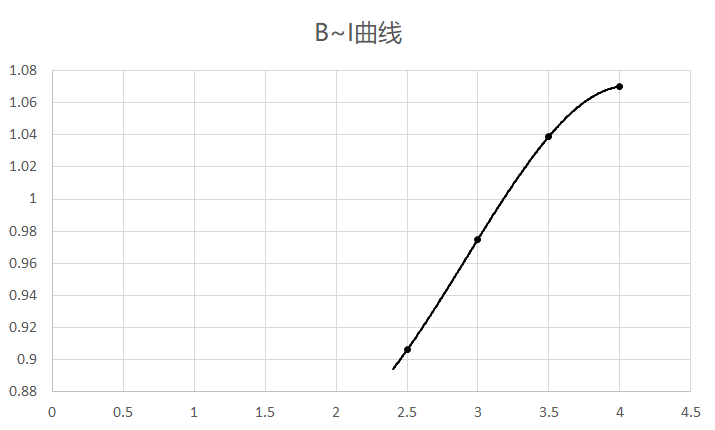
\includegraphics[width=0.75\linewidth]{figure2.png}
\end{figure}

\section{误差分析}
\begin{clause}
	\item 调节过程精密光学仪器易受外界因素影响,观察测量时人眼视觉疲劳,产生较大的随机误差.
	\item 实验过程中流过电磁铁的电流可能产生变化,建议在测量前后分别记录一次电流,在计算时取平均值.
\end{clause}


\section{思考题}
\subsection*{1.}
缓慢转动偏振片,观察到三条圆环的是$\pi$成分,观察到六条圆环的是$\sigma$成分.

$\Delta M=+1$时,谱线的频率增加,波长减小,由$2dcos\phi=k\lambda$可得,随$\lambda$减小,$cos\phi$减小,$\phi$增大,故外侧三条圆环为左旋光.同理可得,内侧三条圆环$\Delta M=-1$,为右旋光.

沿着磁场方向观测时,$\Delta M=+1$为左旋光,其频率增加,$\Delta M=-1$为右旋光,其频率减小.

\subsection*{2.}
在常温范围内,随气压$p$增大,空气折射率$n$增大.

由干涉极大条件$2ndcos\phi=k\lambda$可知,相同级次$k$的圆环的入射角$\phi$增大,半径增大,可观察到圆环逐渐扩大.

相邻两组圆环的角间距$\Delta\phi=\frac{\lambda}{2ndsin\phi}$,随$n$增大而减小,可观察到相邻两组圆环间距减小,圆环变密.

\subsection*{3.}
\begin{clause}
	\item 反推能级结构:本实验利用汞546.1mm谱线的上下能级结构推出了其塞曼效应图象,同时也可以通过塞曼效应图象反推并验证原子的能级结构.
	\item 计算朗德因子:由公式$\Delta \tilde{v}=(M_2g_2-M_1g_1)\frac{e}{4\pi mc}B=(M_2g_2-M_1g_1)L$和$\Delta \tilde{v}=\tilde{v_b}-\tilde{v_a}=\frac{\Delta D_{ab}^2}{2d\Delta D^2}$,可通过塞曼效应测得的$B$、$D_k$、$D_{k-1}$、$D_a$、$D_b$来计算对应能级的朗德因子$g$.
\end{clause}

\section{实验小结}
本次实验的对观察读数的要求比较高,测量得到的数据也比较多,但数据处理相对比较简单.光学仪器都属于比较精密的仪器,需要我们耐心细致地进行调节,完全按照要求进行操作,学会熟练使用测微目镜.在实验中我遇到的较大问题就是对测微目镜的使用不熟悉,没有搞清应该对准刻度线的哪个位置进行读数.再次感谢助教的悉心指导!

\newpage
\section{原始数据表格}

\end{document}